\section{Data to Monte Carlo comparisons at $\sqrt{s}=900$ GeV in
  Minimum Bias events}
\label{sc:DataVsMCMB900}

In this section we present the comparison of several calorimeter-based
distributions in data with {\sc pythia} Mininimum Bias Monte Carlo simulation. All distributions
shown in this section are required to pass the event selections
described in Sec.4. The Monte Carlo distributions shown in this section
are normalized so that the total number of events in Monte Carlo sample
mathces the number of events observed in data.


\subsection{Basic $\etmiss$-related distributions}
\begin{figure}[h!]
 \centering
 \begin{tabular}{ll}
  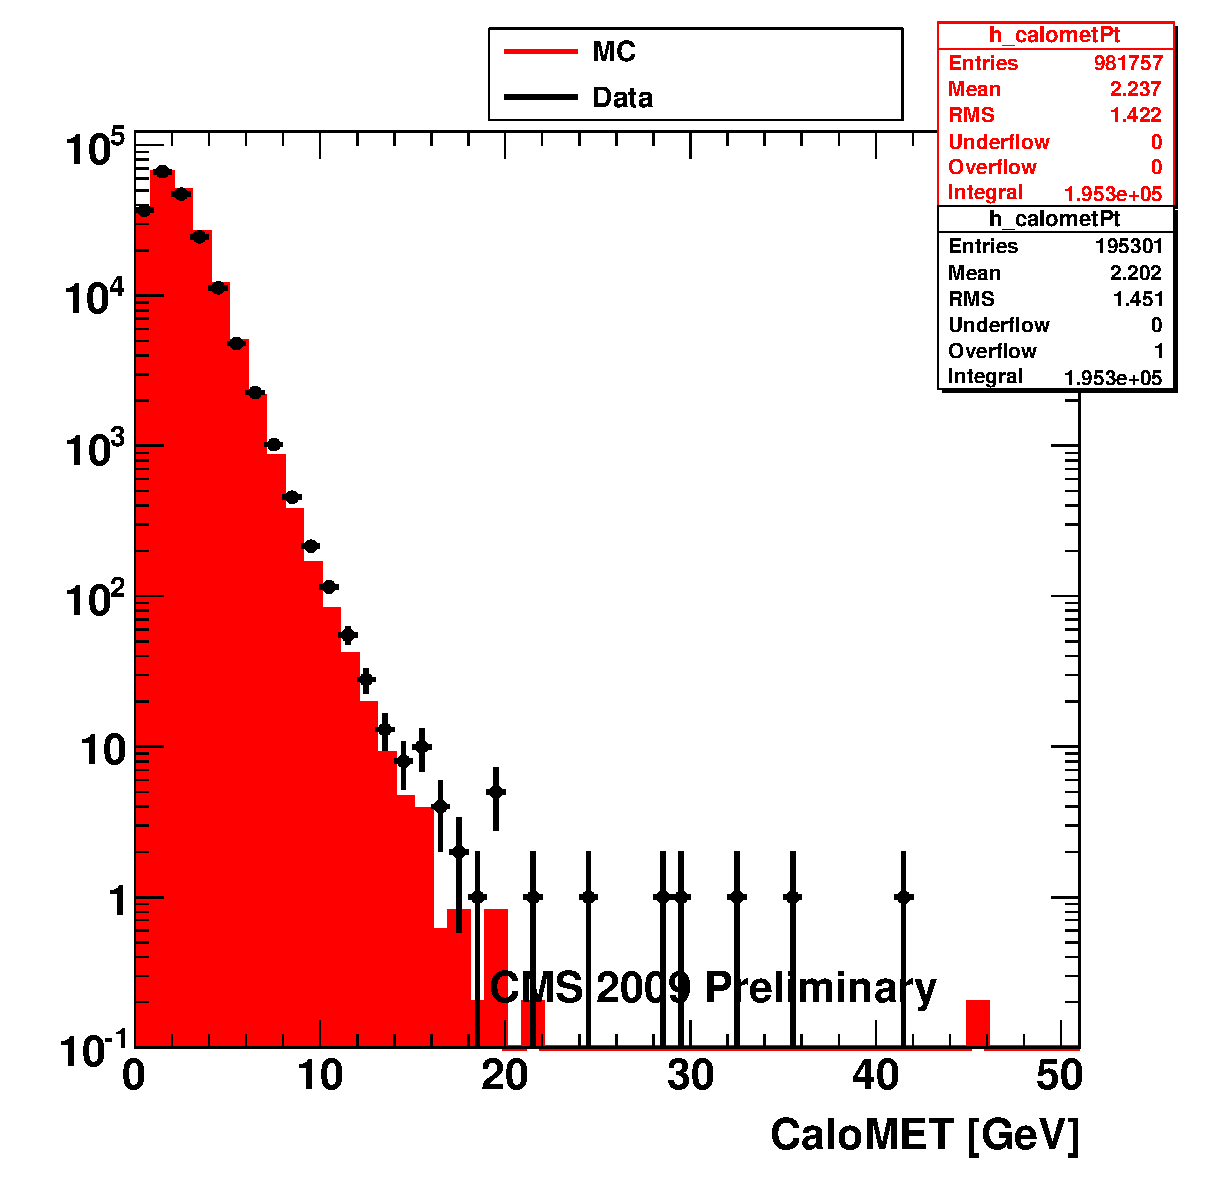
\includegraphics[width=0.40\textwidth]{plots_DataVsMC_MB_900GeV/h_calometPt.eps} &
  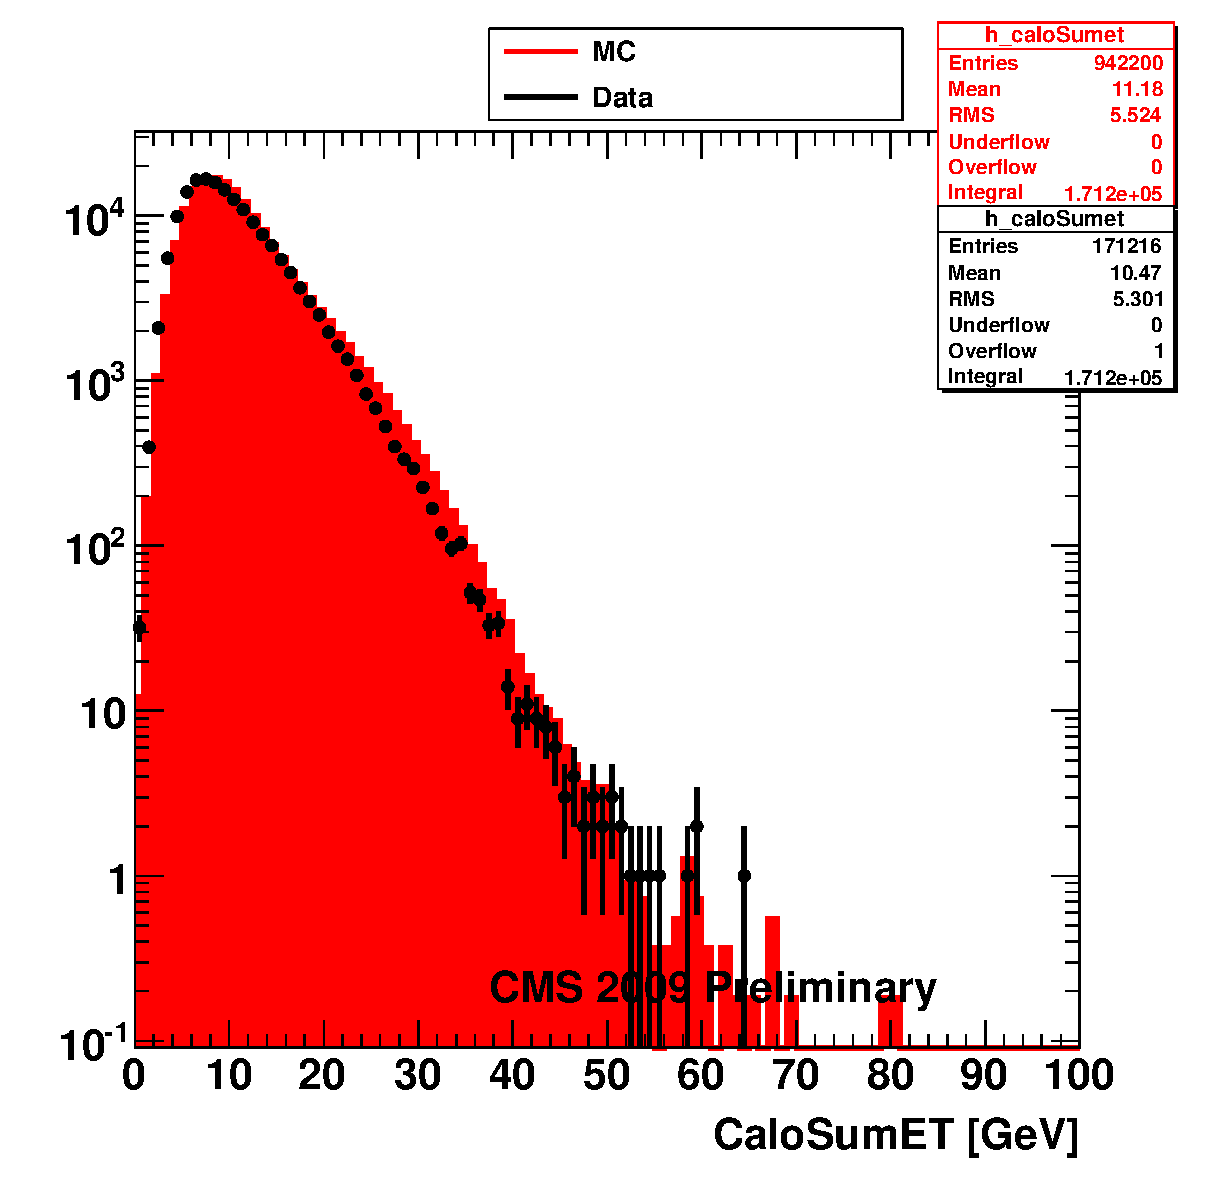
\includegraphics[width=0.40\textwidth]{plots_DataVsMC_MB_900GeV/h_caloSumet.eps} \\
 \end{tabular}
 \caption{$\etmiss$ and SumET distributions in 900 GeV data compared
   with Monte Carlo simulation.
          \label{fig:DataVsMC_MB_900_1}}
\end{figure}

\begin{figure}[h!]
 \centering
 \begin{tabular}{ll}
  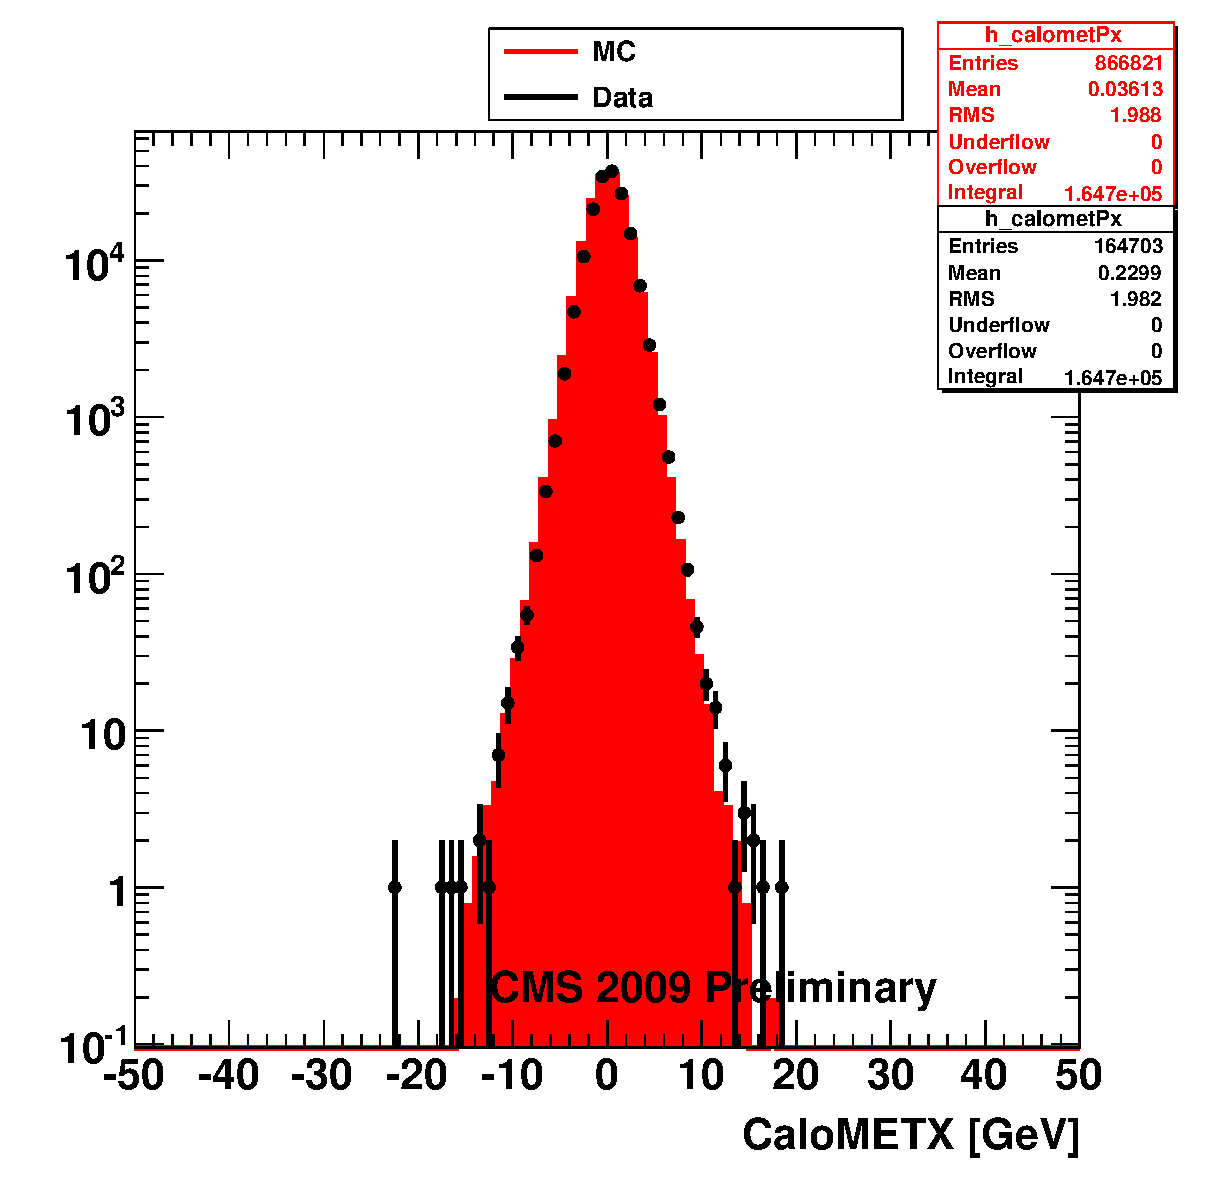
\includegraphics[width=0.40\textwidth]{plots_DataVsMC_MB_900GeV/h_calometPx.eps} &
  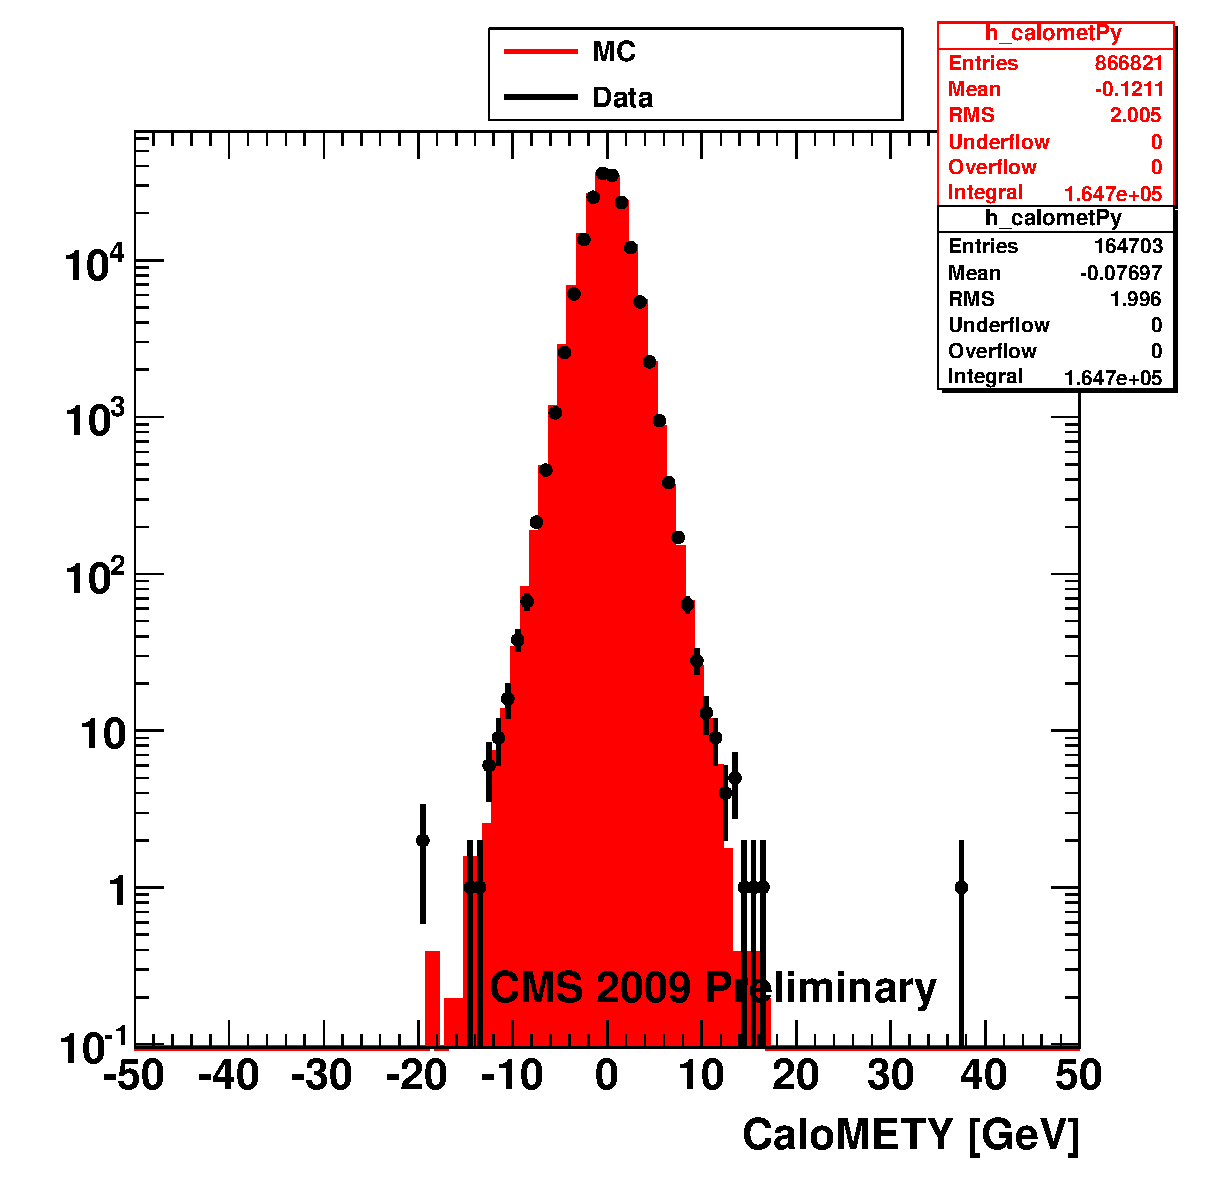
\includegraphics[width=0.40\textwidth]{plots_DataVsMC_MB_900GeV/h_calometPy.eps} \\
 \end{tabular}
 \caption{$\exmiss$ and $\eymiss$ distributions in 900 GeV data compared
   with Monte Carlo simulation.
          \label{fig:DataVsMC_MB_900_2}}
\end{figure}

\begin{figure}[h!]
 \centering
 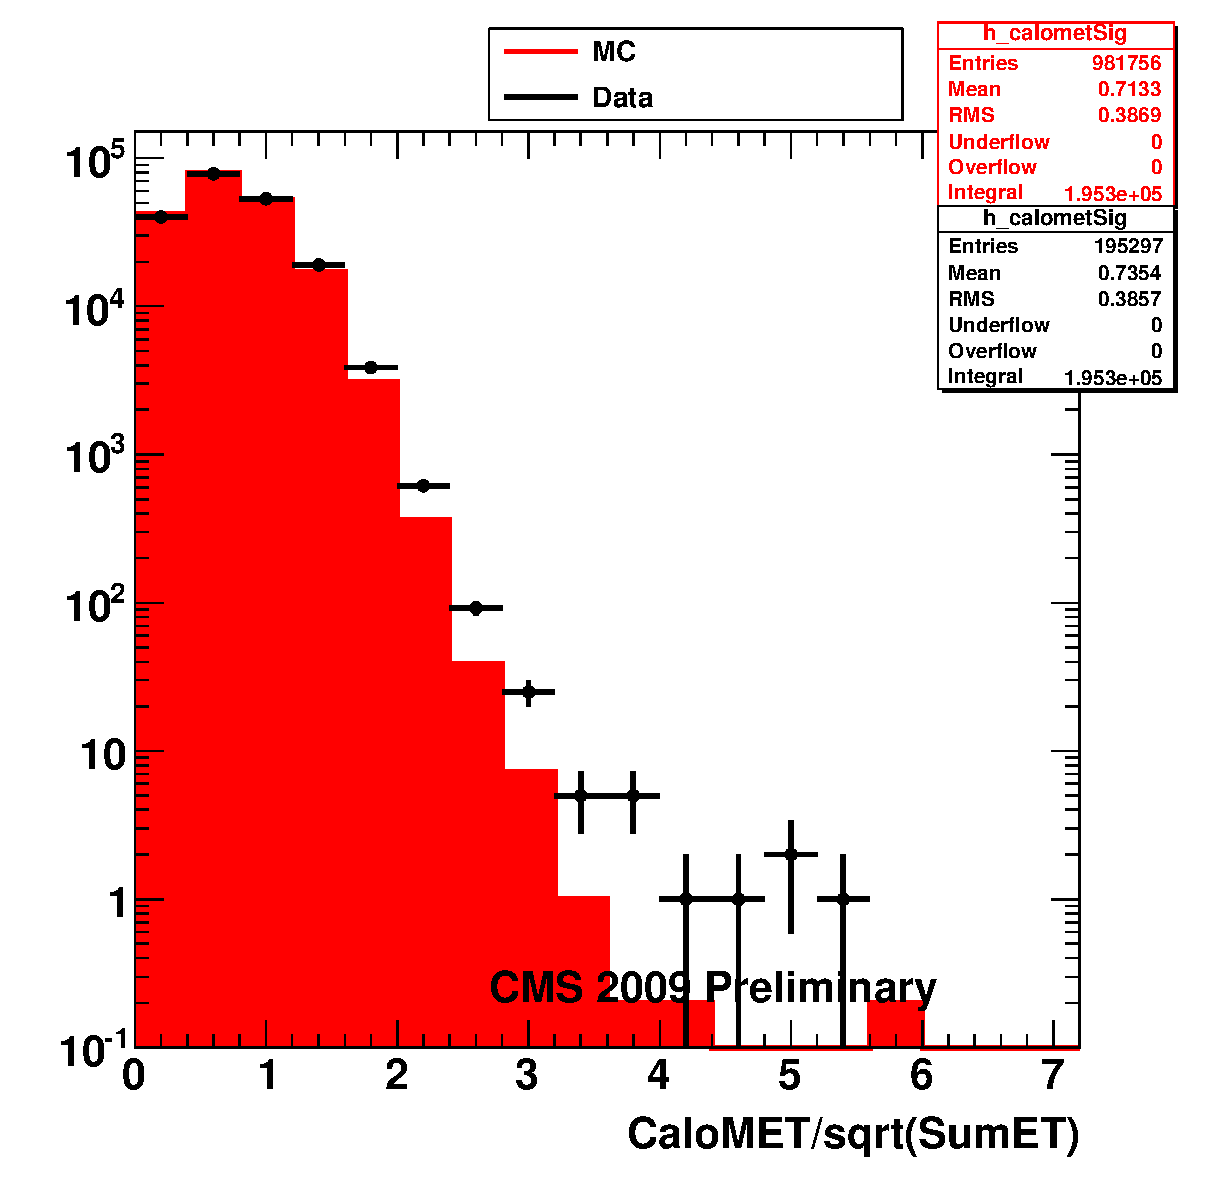
\includegraphics[width=0.40\textwidth]{plots_DataVsMC_MB_900GeV/h_calometSig.eps}
\caption{$\etmiss^{Sig}=\etmiss/\sqrt{SumET}$ distributions in 900 GeV data compared
   with Monte Carlo simulation.
          \label{fig:DataVsMC_MB_900_3}}
\end{figure}

\begin{figure}[h!]
 \centering
 \begin{tabular}{ll}
  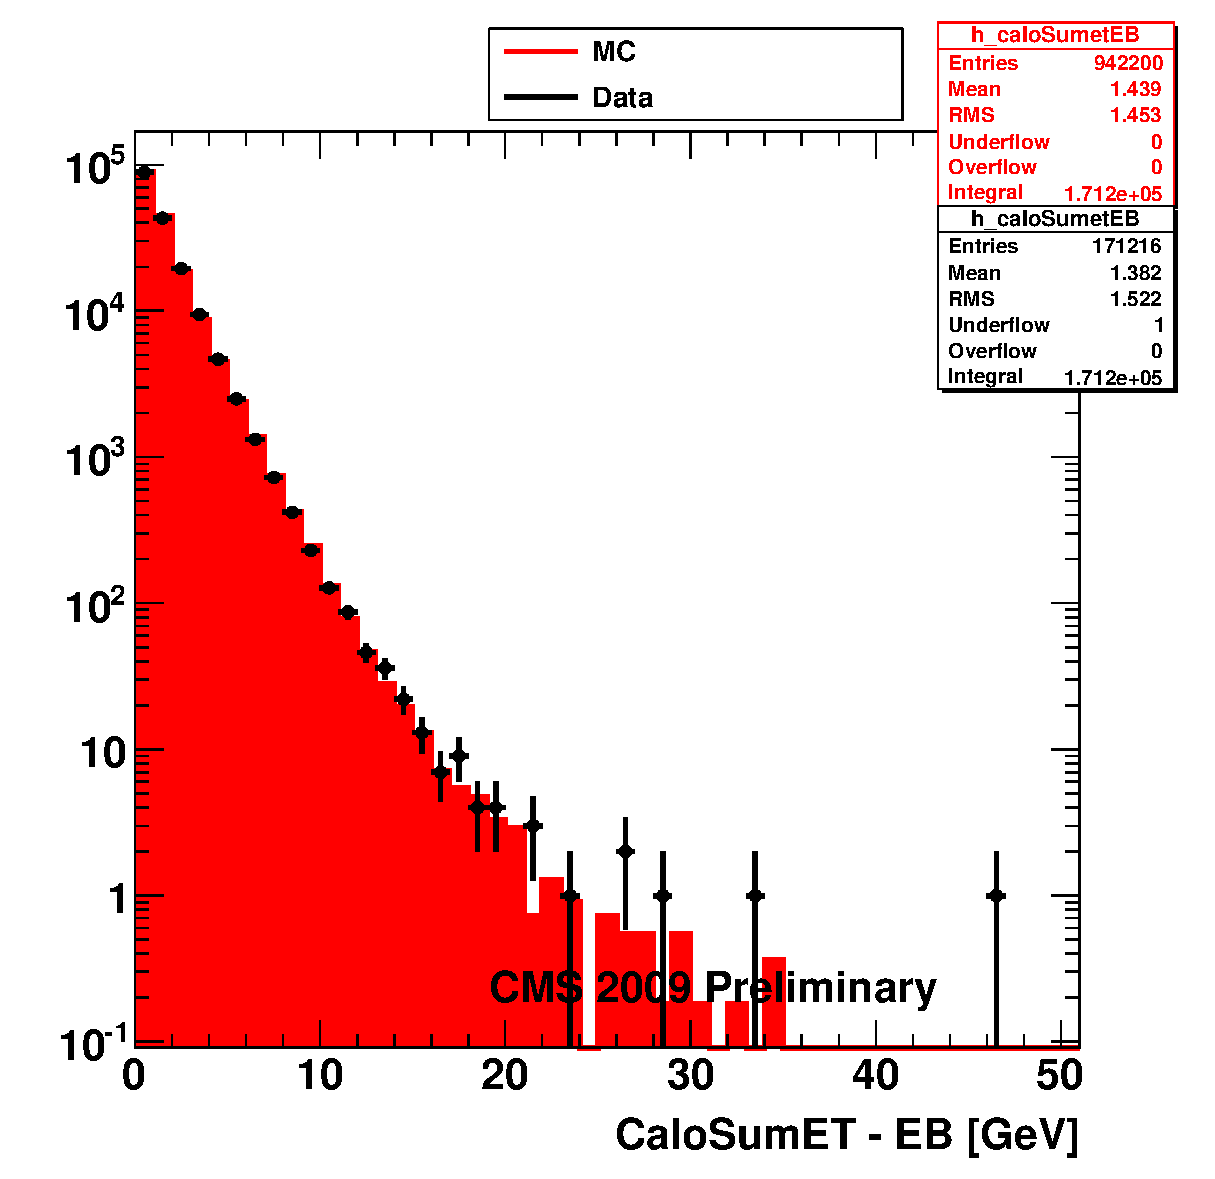
\includegraphics[width=0.40\textwidth]{plots_DataVsMC_MB_900GeV/h_caloSumetEB.eps} &
  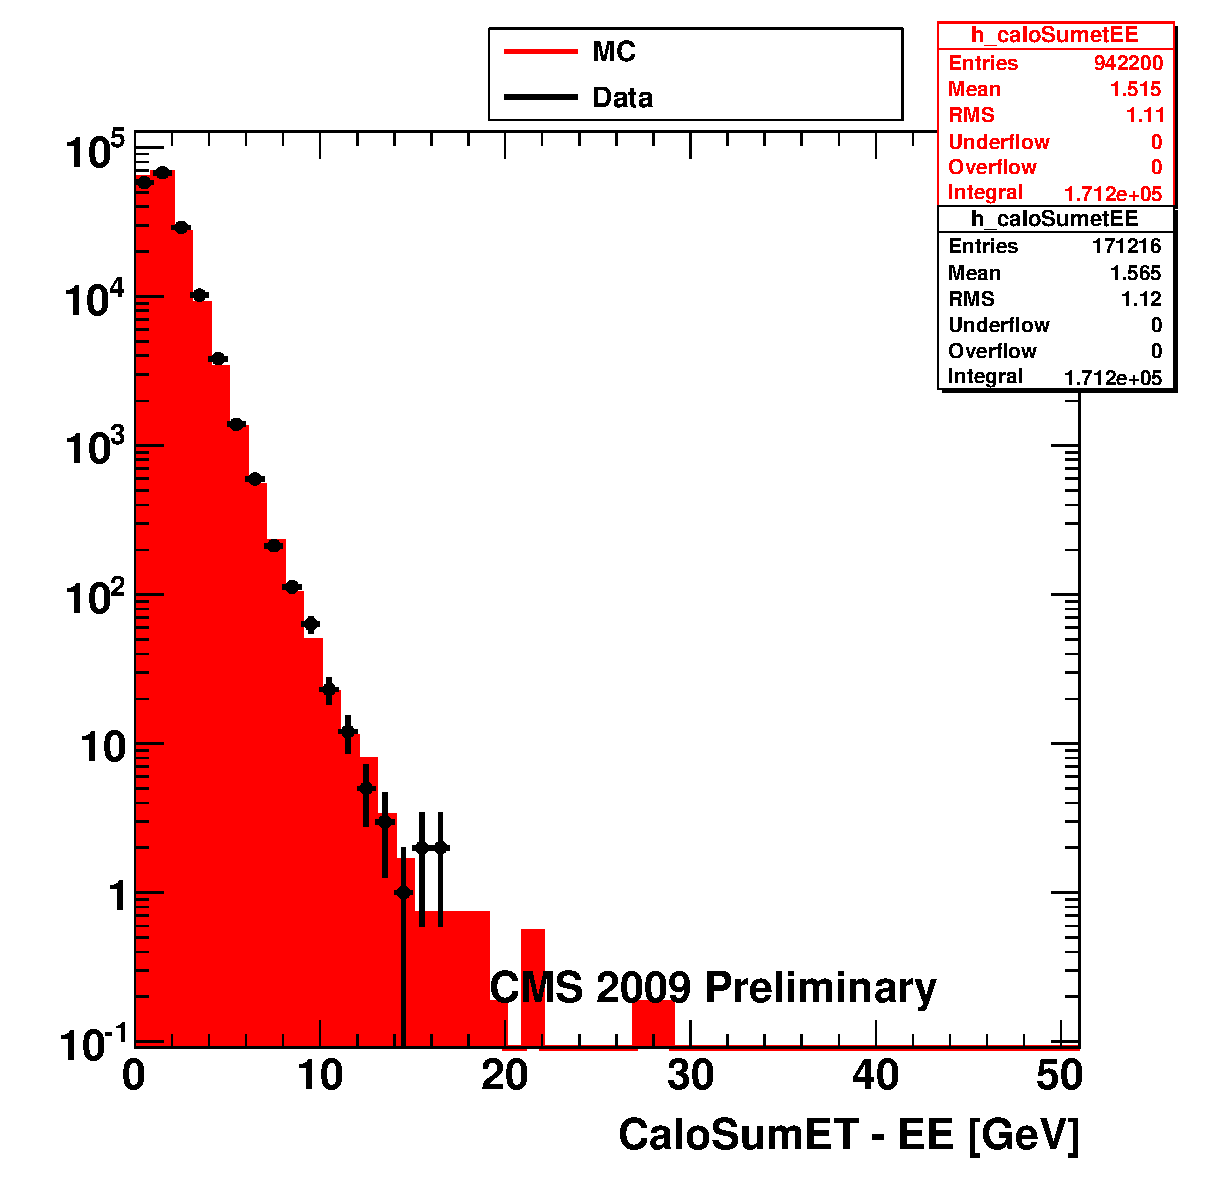
\includegraphics[width=0.40\textwidth]{plots_DataVsMC_MB_900GeV/h_caloSumetEE.eps} \\
 \end{tabular}
 \caption{SumET in ECAL barrel and endcap in 900 GeV data compared
   with Monte Carlo simulation.
          \label{fig:DataVsMC_MB_900_4}}
\end{figure}

\begin{figure}[h!]
 \centering
 \begin{tabular}{ll}
  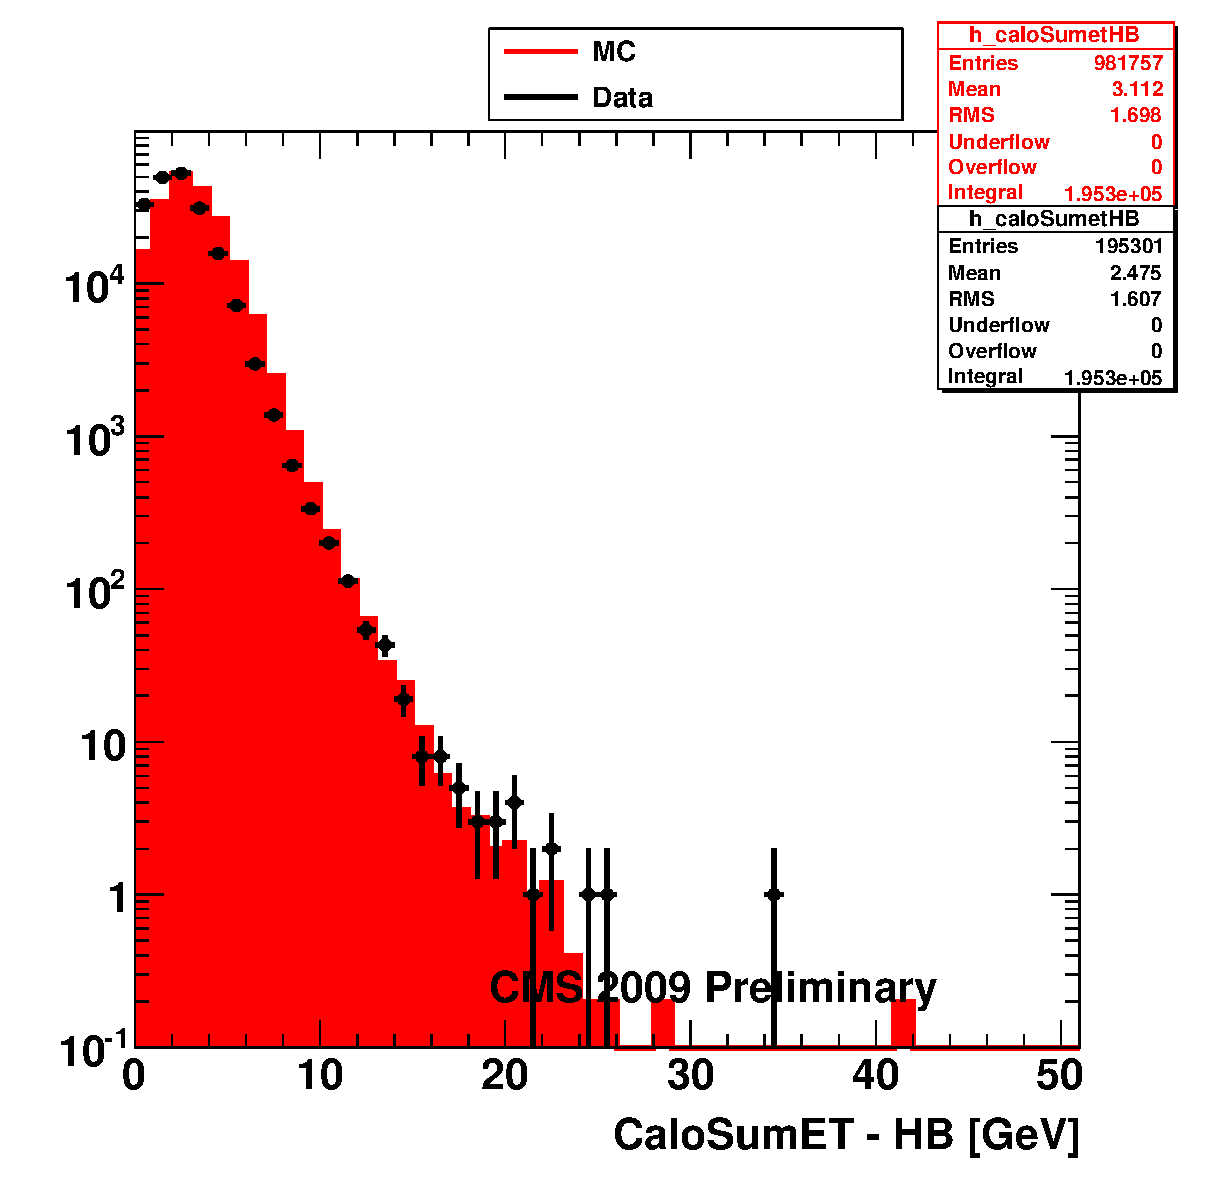
\includegraphics[width=0.40\textwidth]{plots_DataVsMC_MB_900GeV/h_caloSumetHB.eps} &
  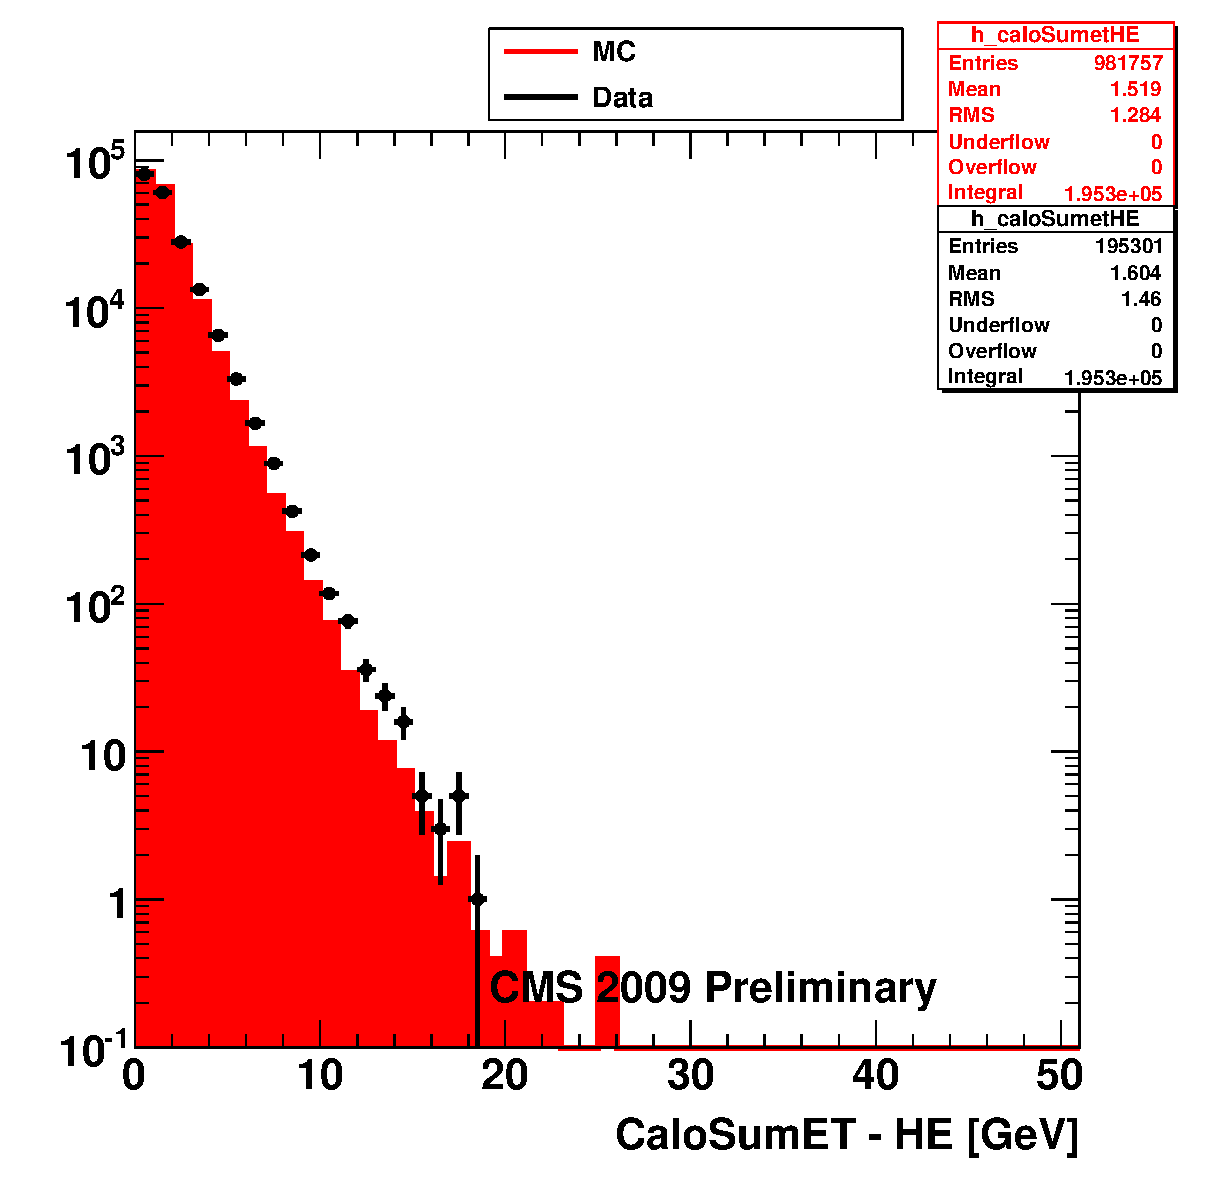
\includegraphics[width=0.40\textwidth]{plots_DataVsMC_MB_900GeV/h_caloSumetHE.eps} \\
 \end{tabular}
 \caption{SumET in HCAL barrel and endcap in 900 GeV data compared
   with Monte Carlo simulation.
          \label{fig:DataVsMC_MB_900_5}}
\end{figure}

\begin{figure}[h!]
 \centering
 \begin{tabular}{ll}
  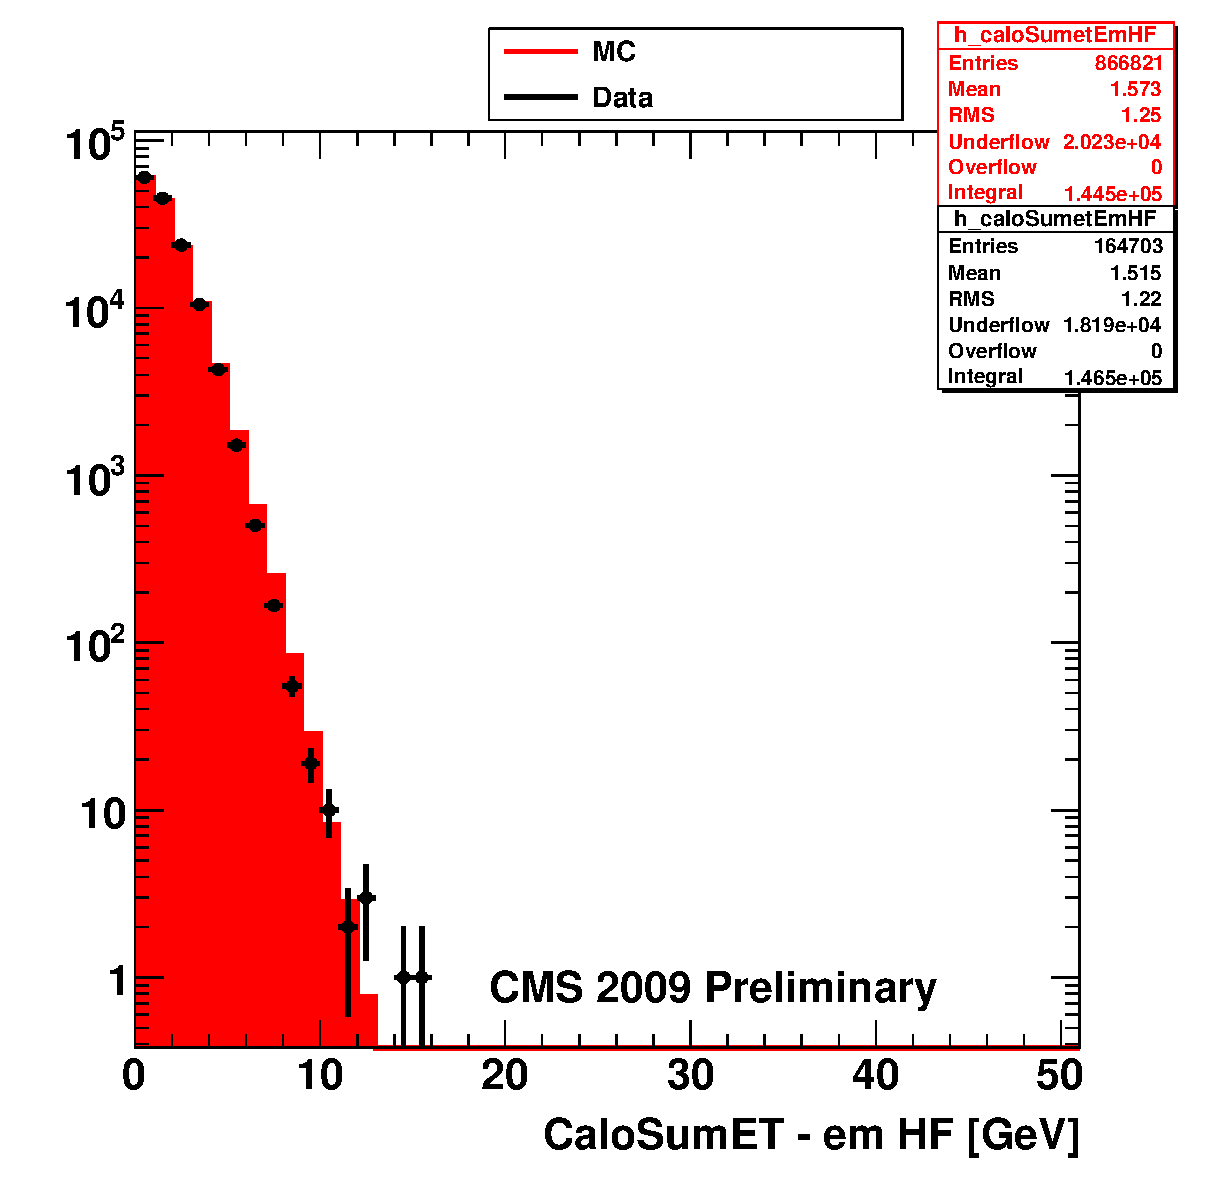
\includegraphics[width=0.40\textwidth]{plots_DataVsMC_MB_900GeV/h_caloSumetEmHF.eps} &
  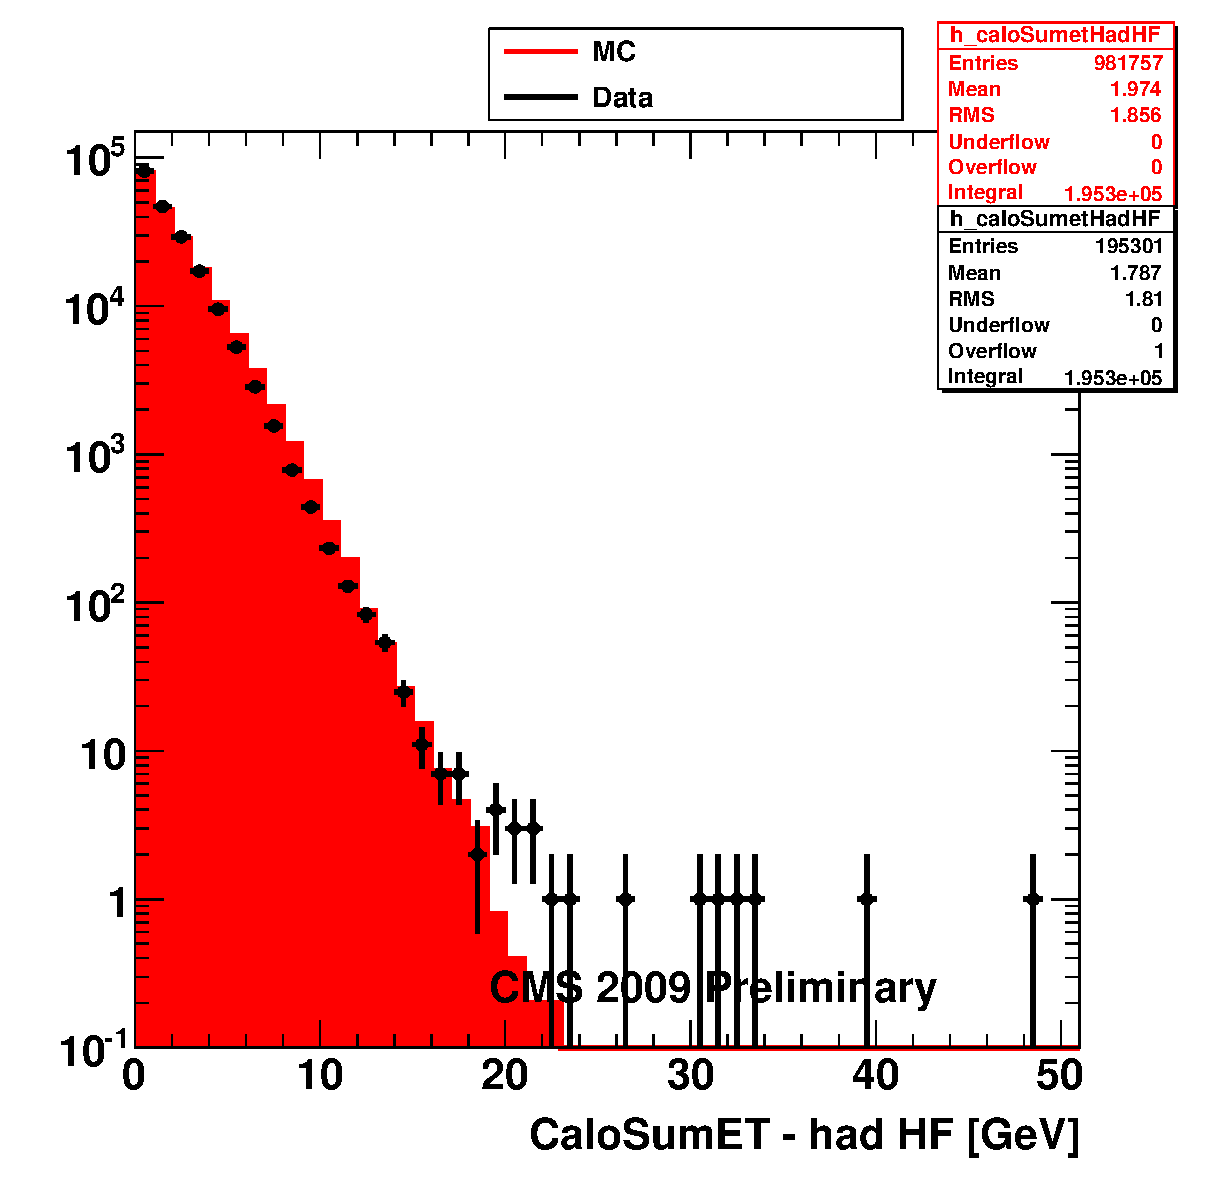
\includegraphics[width=0.40\textwidth]{plots_DataVsMC_MB_900GeV/h_caloSumetHadHF.eps} \\
 \end{tabular}
 \caption{SumET in HF in electromagnetic and hadronic parts in 900 GeV data compared
   with Monte Carlo simulation.
          \label{fig:DataVsMC_MB_900_6}}
\end{figure}

\clearpage

\subsection{$\etmiss$ resolution}

For events with no $\etmiss$ from physics sources, the $\etmiss$ resolution can be most generally parameterized
according to the following expression (CMS AN-2007/041):
\begin{equation}
  \sigma\left(\etmiss\right)=A \oplus B\sqrt{\sum E_\text{T}-D} \oplus C\left(\sum E_\text{T}-D\right),
  \label{eq:MET_sigma}
\end{equation}
where $A$ is the noise term, $B$ is the stohastic term, $C$ is the constant term, and $D$ is the offset term. In such events
$\exmiss$ and $\eymiss$ are expected to follow a Gaussian distribution with the mean of zero and the standard deviation
of $\sigma$. It can also be shown that $\sigma\left(\etmiss\right)$ is proportional to this $\sigma$. Therefore,
by looking at $\sigma\left(\exmiss\right)$ and $\sigma\left(\eymiss\right)$ as a function of $\sum E_\text{T}$ it is possible to
study the $\etmiss$ resolution and the relative contributions of different resolution terms at different values of $\sum E_\text{T}$.
Figure~\ref{fig:MExySigma_vs_SumET_900} shows the $\sigma\left(\exmiss\right)$ and $\sigma\left(\eymiss\right)$ 
vs. $\sum E_\text{T}$ for 900 GeV data compared with Monte Carlo simulation. $\sigma\left(\exmiss\right)$ and $\sigma\left(\eymiss\right)$
were extracted from a Gaussian fit to $\exmiss$ and $\eymiss$ distributions, respectively, in a region of $\pm 1.5$ RMS around the mean.
Figures~\ref{fig:MExSigma_vs_SumET_900_fit} and \ref{fig:MEySigma_vs_SumET_900_fit} show the fit of $\sigma\left(\exmiss\right)$
 and $\sigma\left(\eymiss\right)$ vs. $\sum E_\text{T}$ to Eq.~\ref{eq:MET_sigma} for data and Monte Carlo at $900$ GeV.
The offset term $D$, which from results presented in Section~\ref{sc:CaloNoise} is expected to be small, had to be fixed to zero in 
order to get a stable fit.

\begin{figure}[h!]
 \centering
 \begin{tabular}{ll}
  \includegraphics[width=0.5\textwidth]{plots_DataVsMC_MB_900GeV/h_metxsigma_sumet_900.eps} &
  \includegraphics[width=0.5\textwidth]{plots_DataVsMC_MB_900GeV/h_metysigma_sumet_900.eps} \\
 \end{tabular}
 \caption{\small $\sigma\left(\exmiss\right)$ and $\sigma\left(\eymiss\right)$ vs. $\sum E_\text{T}$ for data at $900$ GeV
          compared with Monte Carlo simulation.\label{fig:MExySigma_vs_SumET_900}}
\end{figure}

\begin{figure}[h!]
 \centering
 \begin{tabular}{ll}
  \includegraphics[width=0.5\textwidth]{plots_DataVsMC_MB_900GeV/final_metxsigma_sumet_MC_900.eps} &
  \includegraphics[width=0.5\textwidth]{plots_DataVsMC_MB_900GeV/final_metxsigma_sumet_DATA_900.eps} \\
 \end{tabular}
 \caption{\small Fit of the $\sigma\left(\exmiss\right)$ vs. $\sum E_\text{T}$ for data and Monte Carlo at $900$ GeV. Parameter $D$ in the fit was fixed
          to zero.\label{fig:MExSigma_vs_SumET_900_fit}}
\end{figure}

\begin{figure}[h!]
 \centering
 \begin{tabular}{ll}
  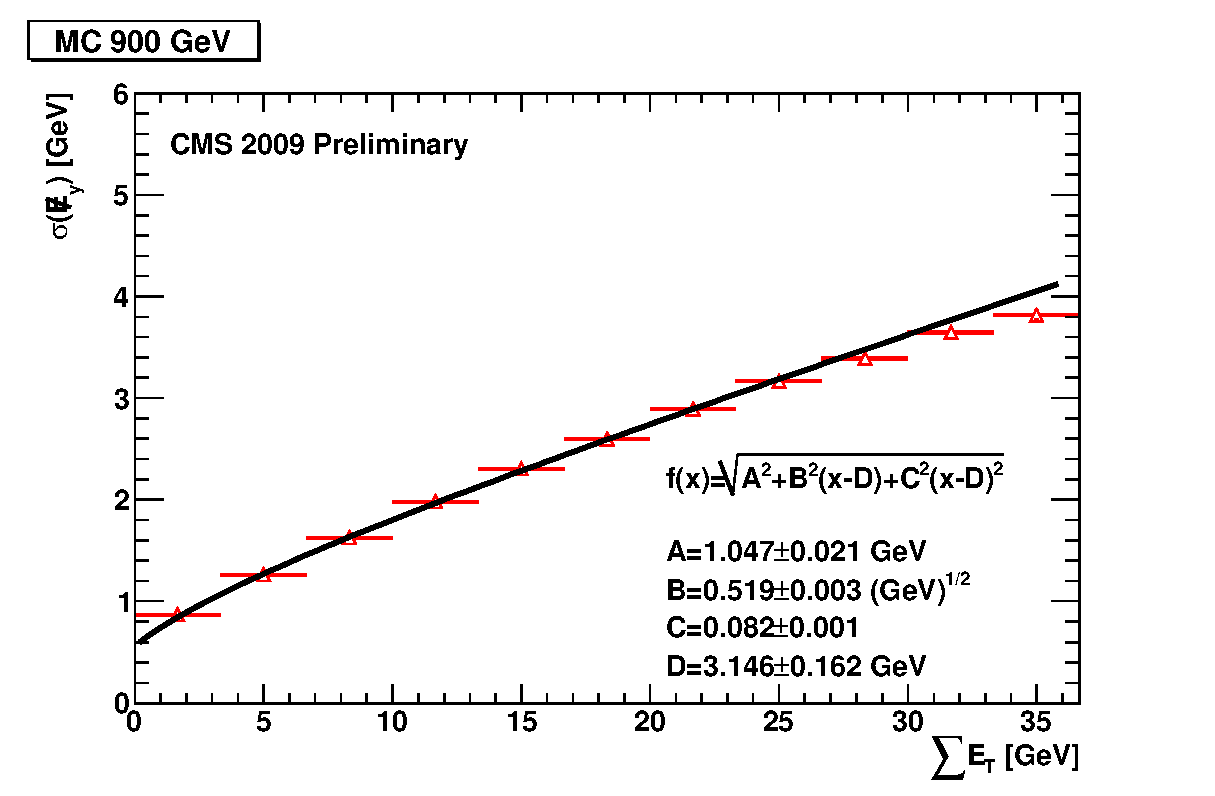
\includegraphics[width=0.5\textwidth]{plots_DataVsMC_MB_900GeV/final_metysigma_sumet_MC_900.eps} &
  \includegraphics[width=0.5\textwidth]{plots_DataVsMC_MB_900GeV/final_metysigma_sumet_DATA_900.eps} \\
 \end{tabular}
 \caption{\small Fit of the $\sigma\left(\eymiss\right)$ vs. $\sum E_\text{T}$ for data and Monte Carlo at $900$ GeV. Parameter $D$ in the fit was fixed
          to zero.\label{fig:MEySigma_vs_SumET_900_fit}}
\end{figure}

\clearpage

\subsection{$\etmiss$ and SumET dependence on $\eta$}

\begin{figure}[h!]
 \centering
 \begin{tabular}{ll}
  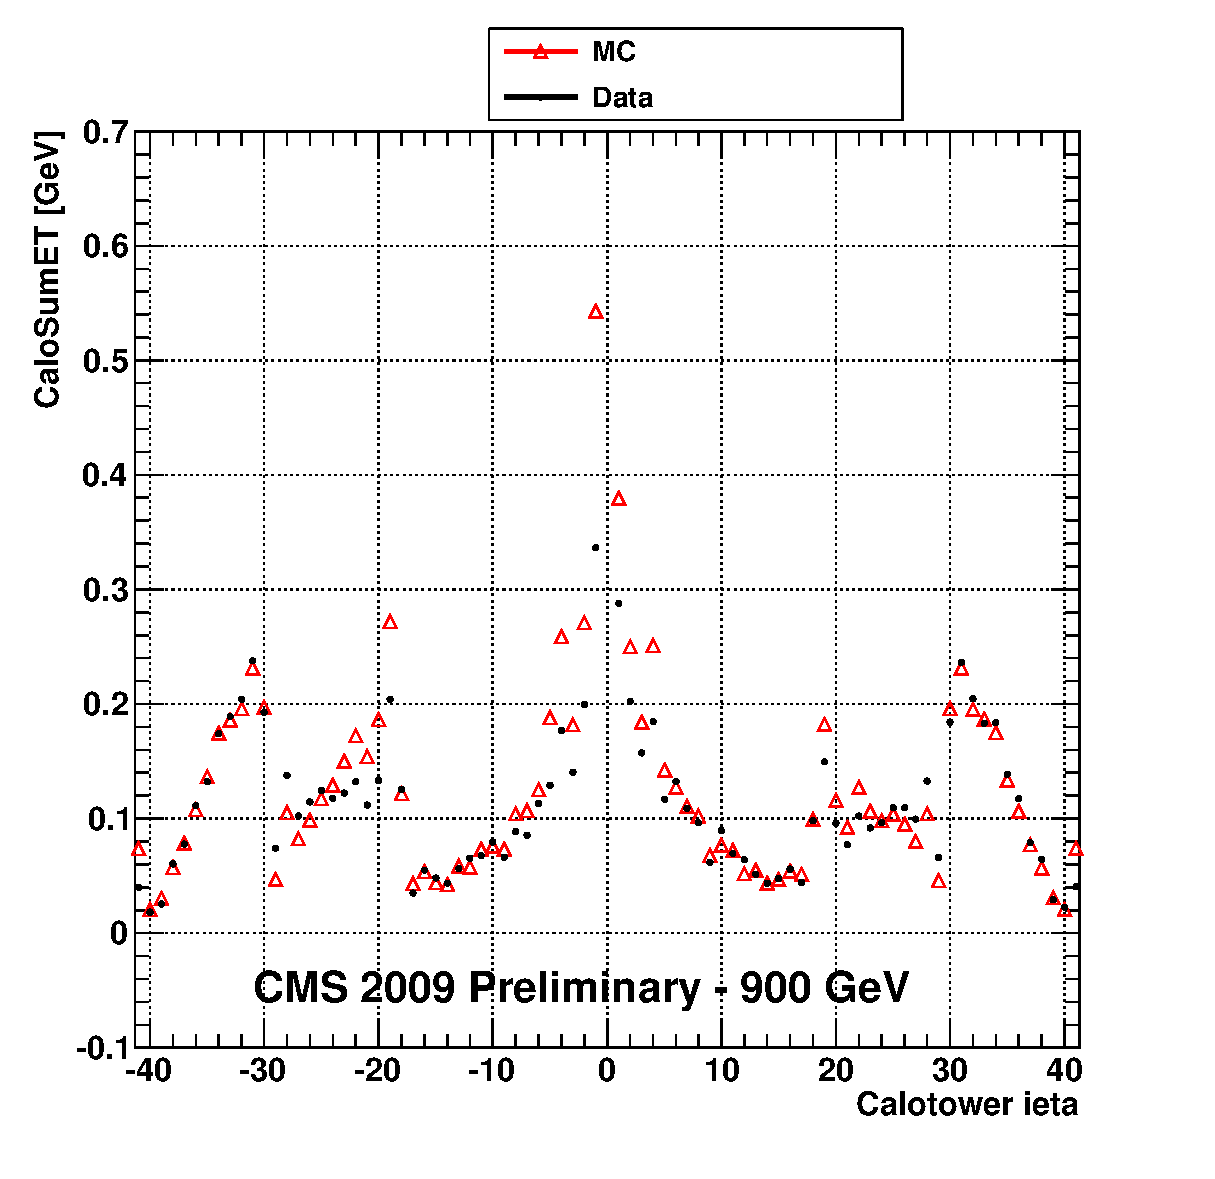
\includegraphics[width=0.5\textwidth]{plots_DataVsMC_MB_900GeV/g_caloSumetMean_vs_ieta_900.eps} &
  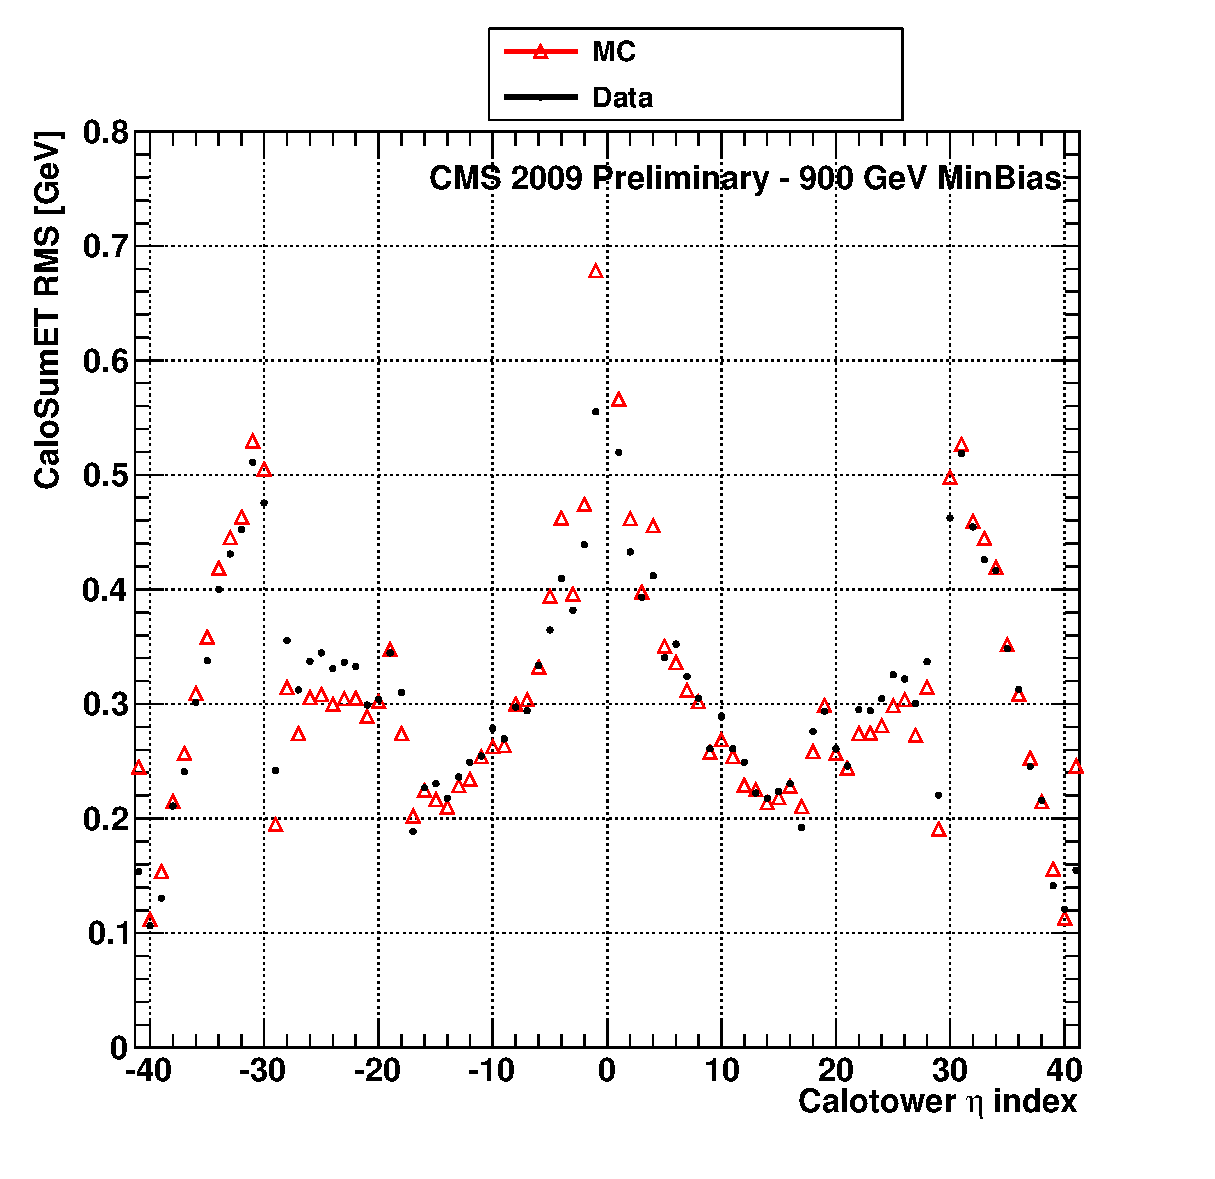
\includegraphics[width=0.5\textwidth]{plots_DataVsMC_MB_900GeV/g_caloSumetRMS_vs_ieta_900.eps} \\
 \end{tabular}
 \caption{\small Comparison of the SumET Mean vs. i$\eta$ of calotowers and SumET RMS vs. i$\eta$ of calotowers between 
          data and Monte Carlo at $900$ GeV.\label{fig:SumET_MeanRMS_vs_ieta_900}}
\end{figure}

\begin{figure}[h!]
 \centering
 \begin{tabular}{ll}
  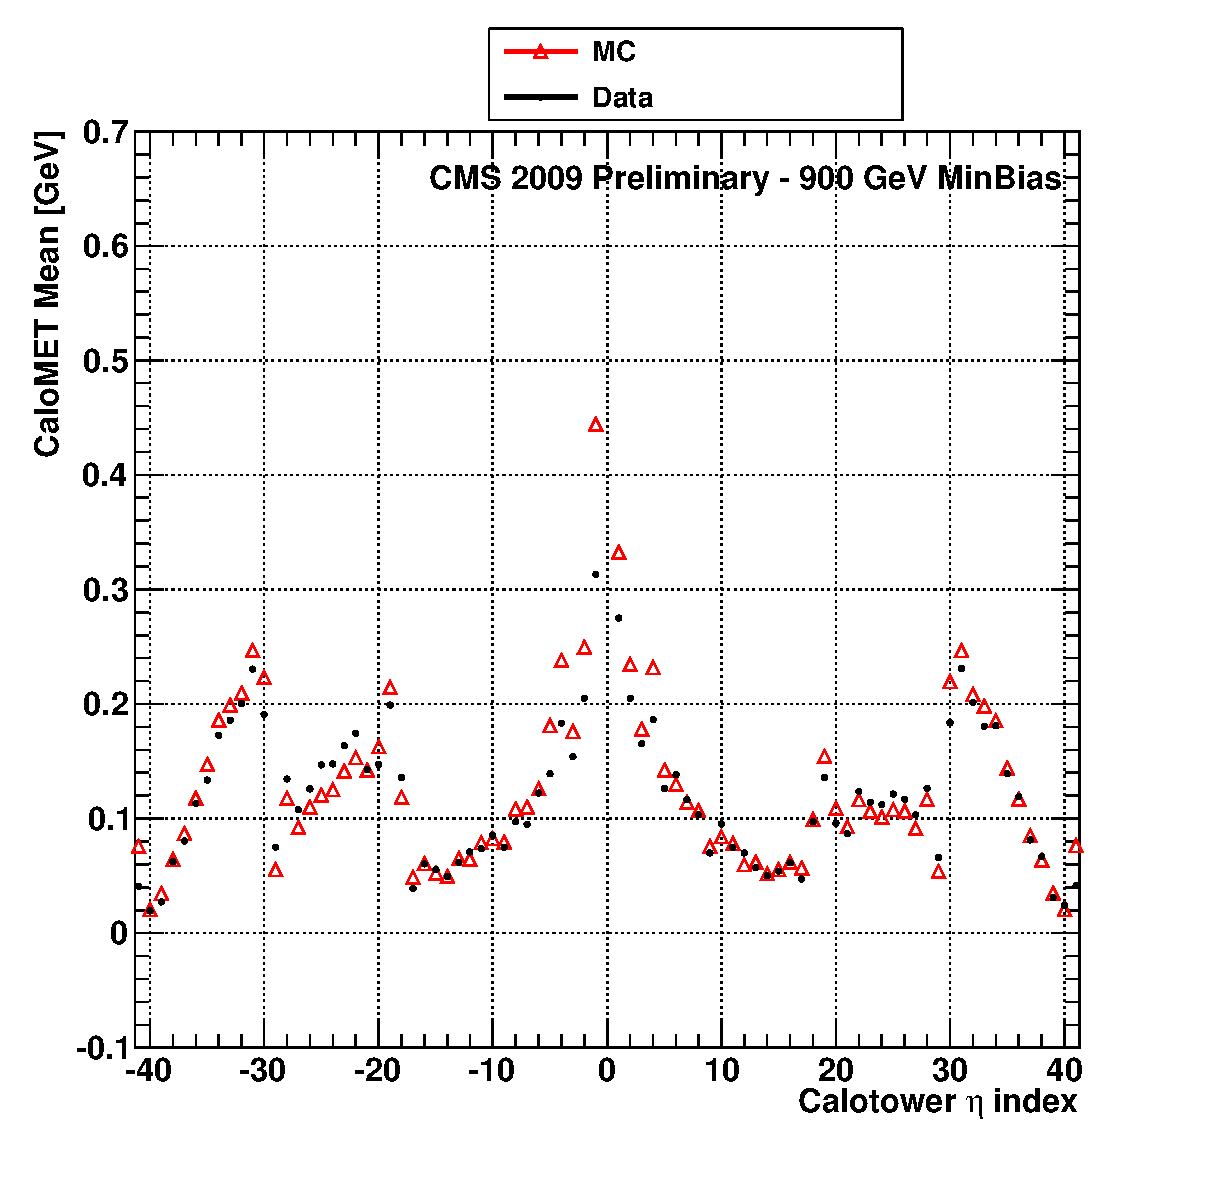
\includegraphics[width=0.5\textwidth]{plots_DataVsMC_MB_900GeV/g_calometPtMean_vs_ieta_900.eps} &
  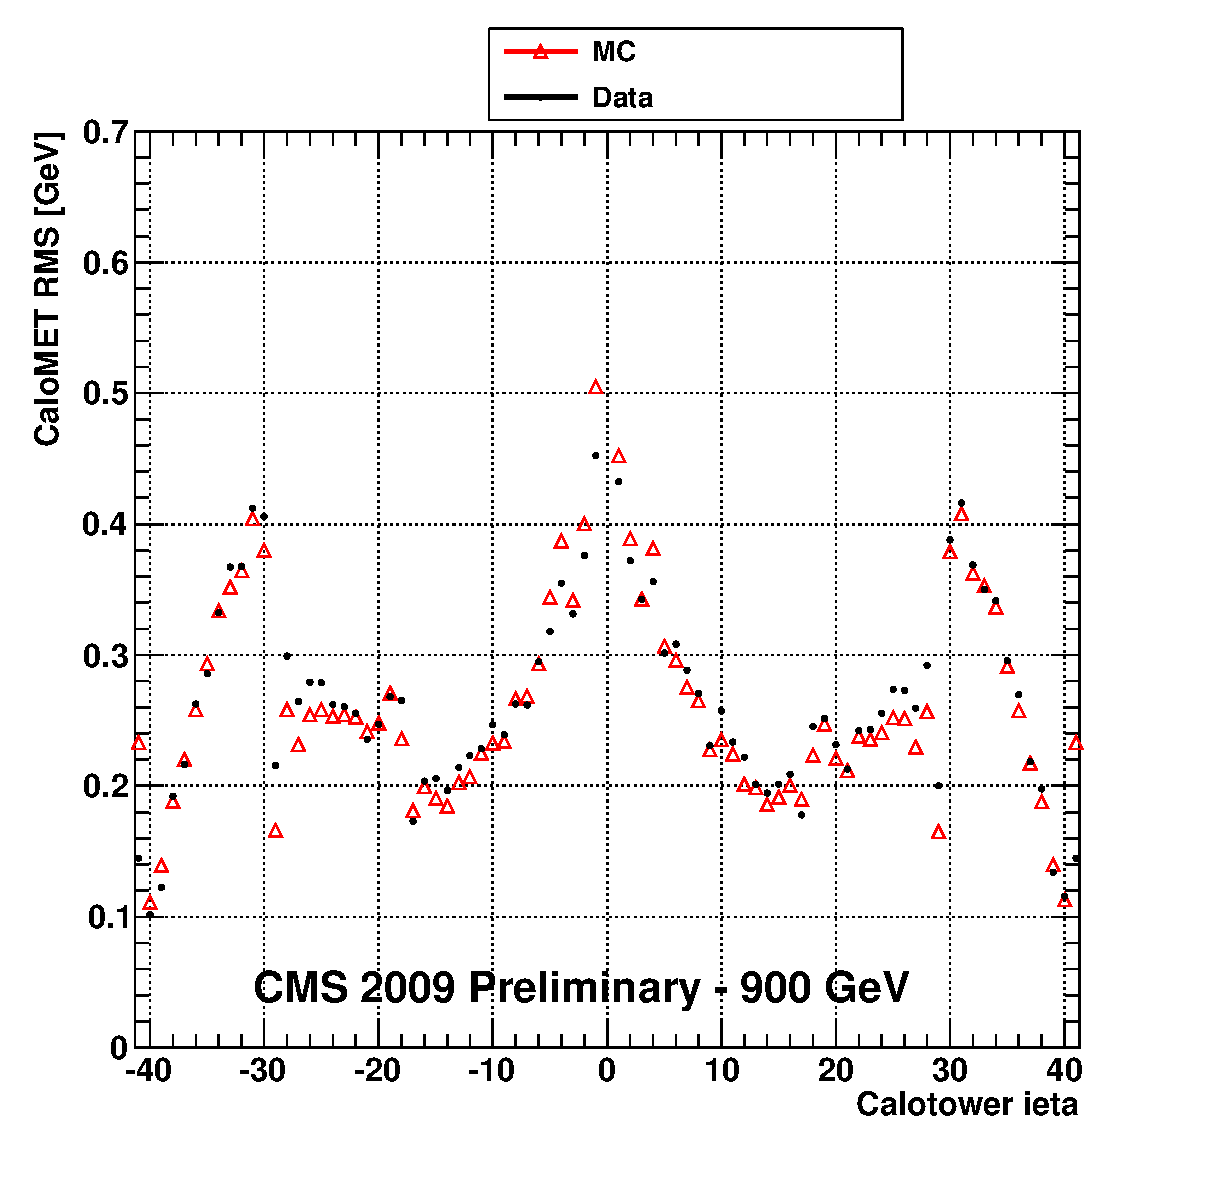
\includegraphics[width=0.5\textwidth]{plots_DataVsMC_MB_900GeV/g_calometPtRMS_vs_ieta_900.eps} \\
 \end{tabular}
 \caption{\small Comparison of the $\etmiss$ Mean vs. i$\eta$ of calotowers and $\etmiss$ RMS vs. i$\eta$ of calotowers between 
          data and Monte Carlo at $900$ GeV.\label{fig:MET_MeanRMS_vs_ieta_900}}
\end{figure}

\begin{figure}[h!]
 \centering
 \begin{tabular}{ll}
  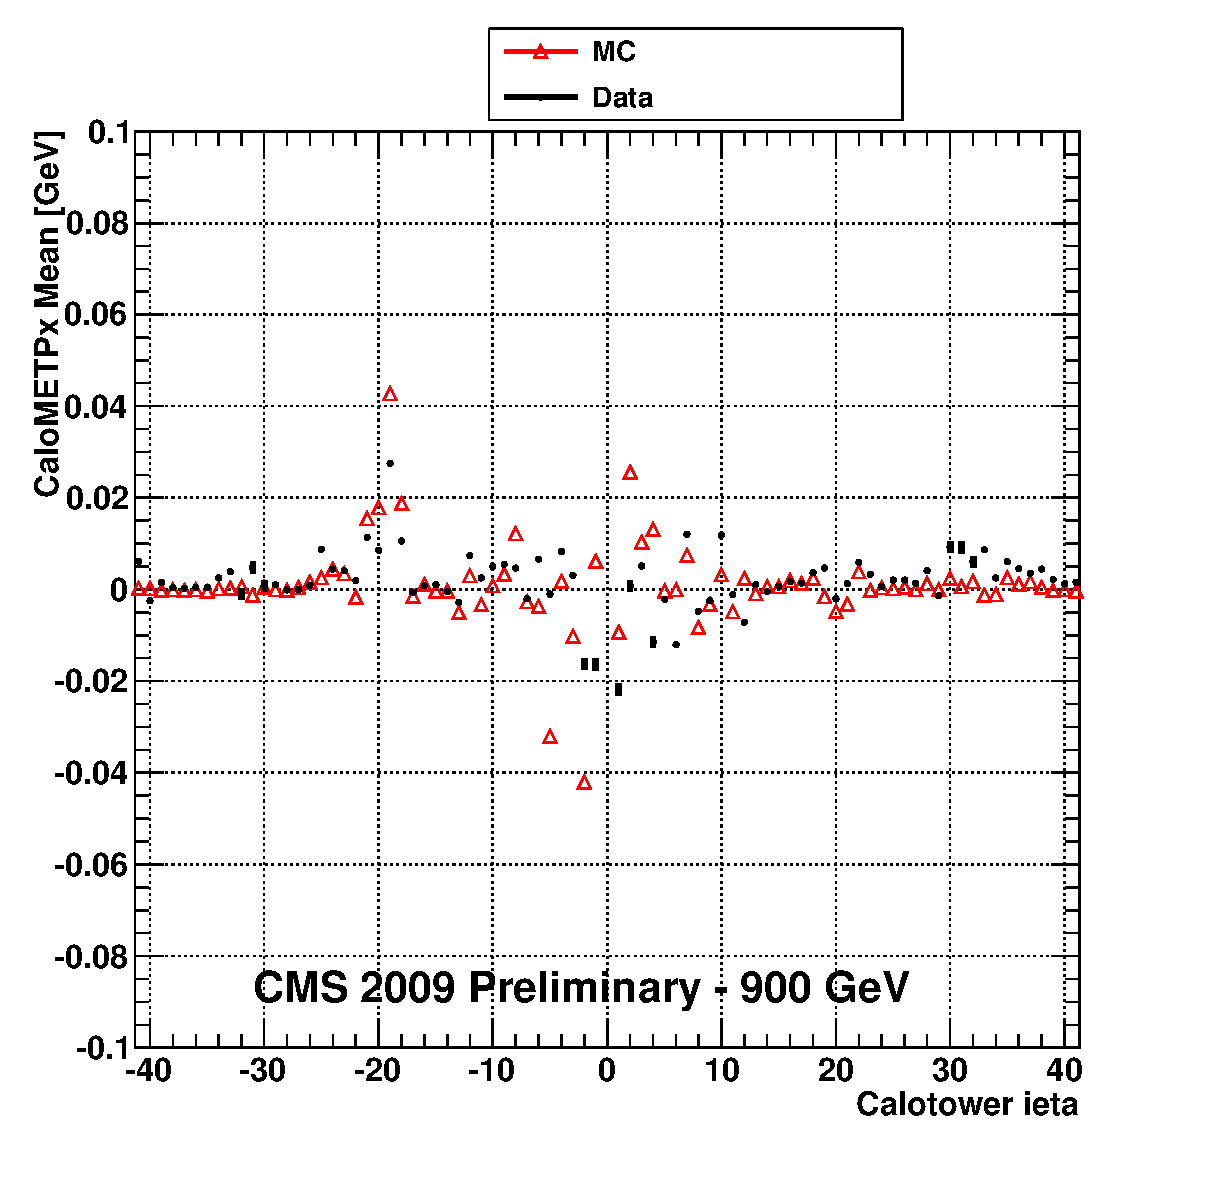
\includegraphics[width=0.5\textwidth]{plots_DataVsMC_MB_900GeV/g_calometPxMean_vs_ieta_900.eps} &
  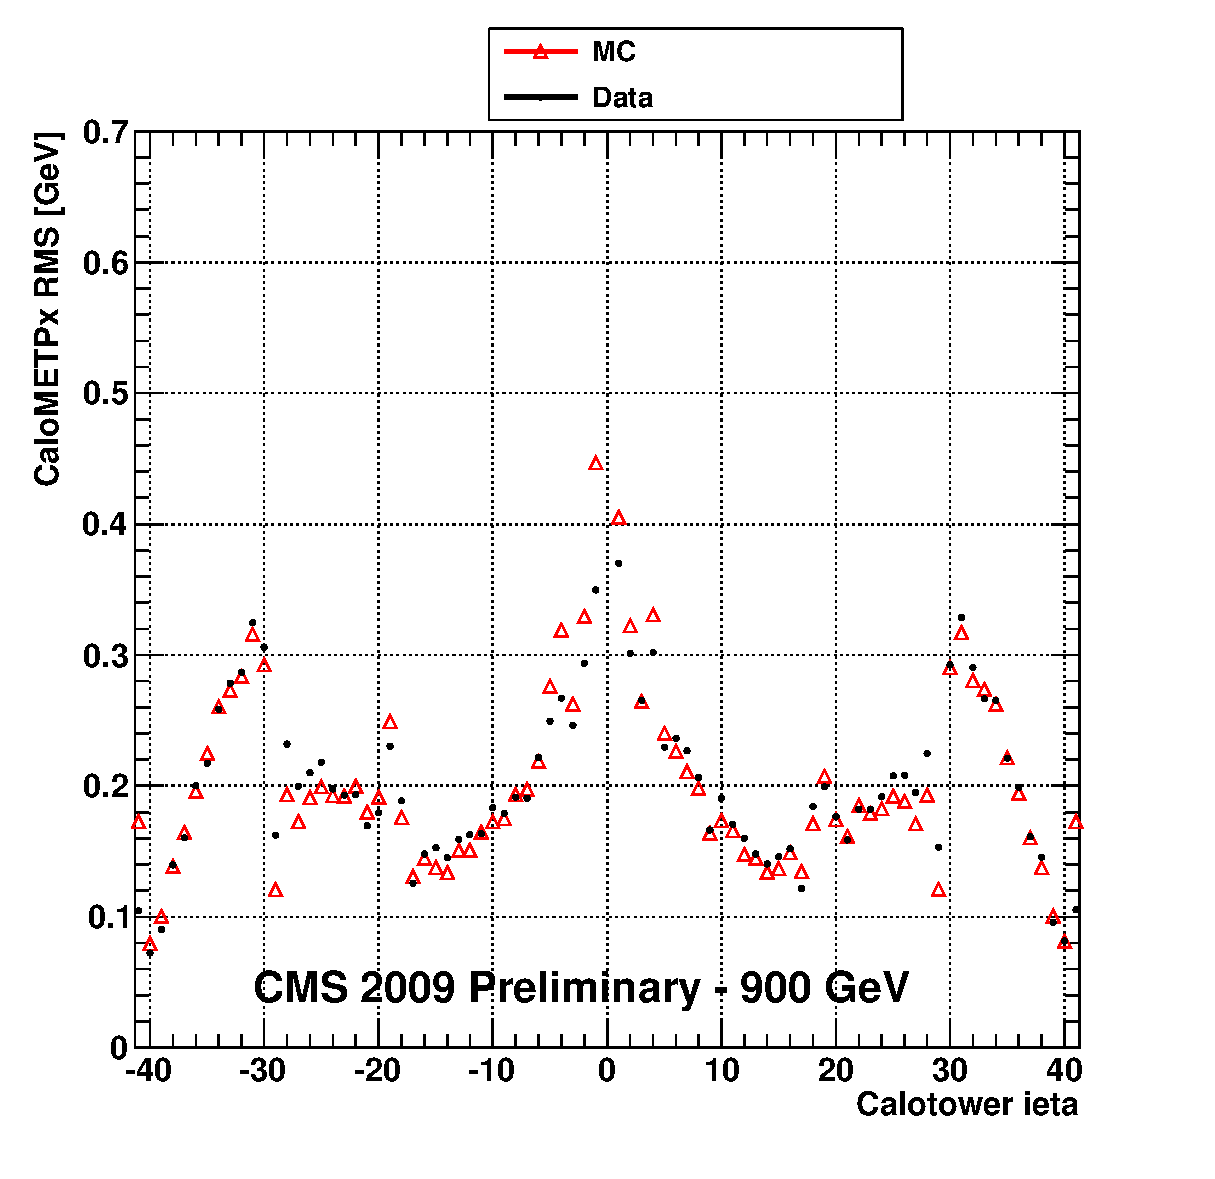
\includegraphics[width=0.5\textwidth]{plots_DataVsMC_MB_900GeV/g_calometPxRMS_vs_ieta_900.eps} \\
 \end{tabular}
 \caption{\small Comparison of the $\exmiss$ Mean vs. i$\eta$ of calotowers and $\exmiss$ RMS vs. i$\eta$ of calotowers between 
          data and Monte Carlo at $900$ GeV.\label{fig:METx_MeanRMS_vs_ieta_900}}
\end{figure}

\begin{figure}[h!]
 \centering
 \begin{tabular}{ll}
  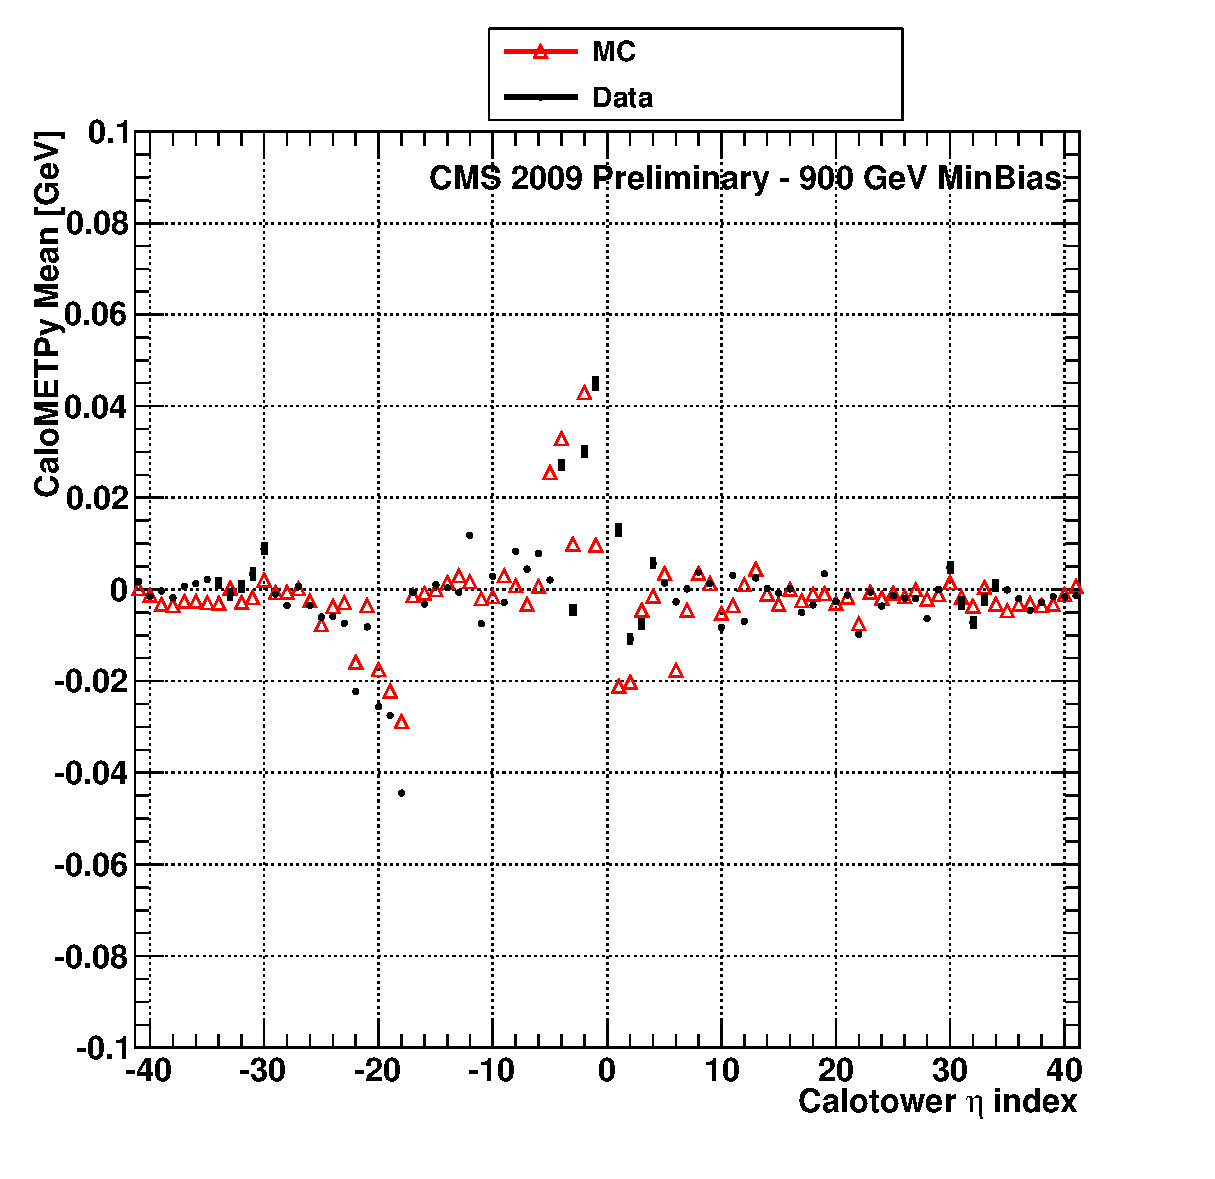
\includegraphics[width=0.5\textwidth]{plots_DataVsMC_MB_900GeV/g_calometPyMean_vs_ieta_900.eps} &
  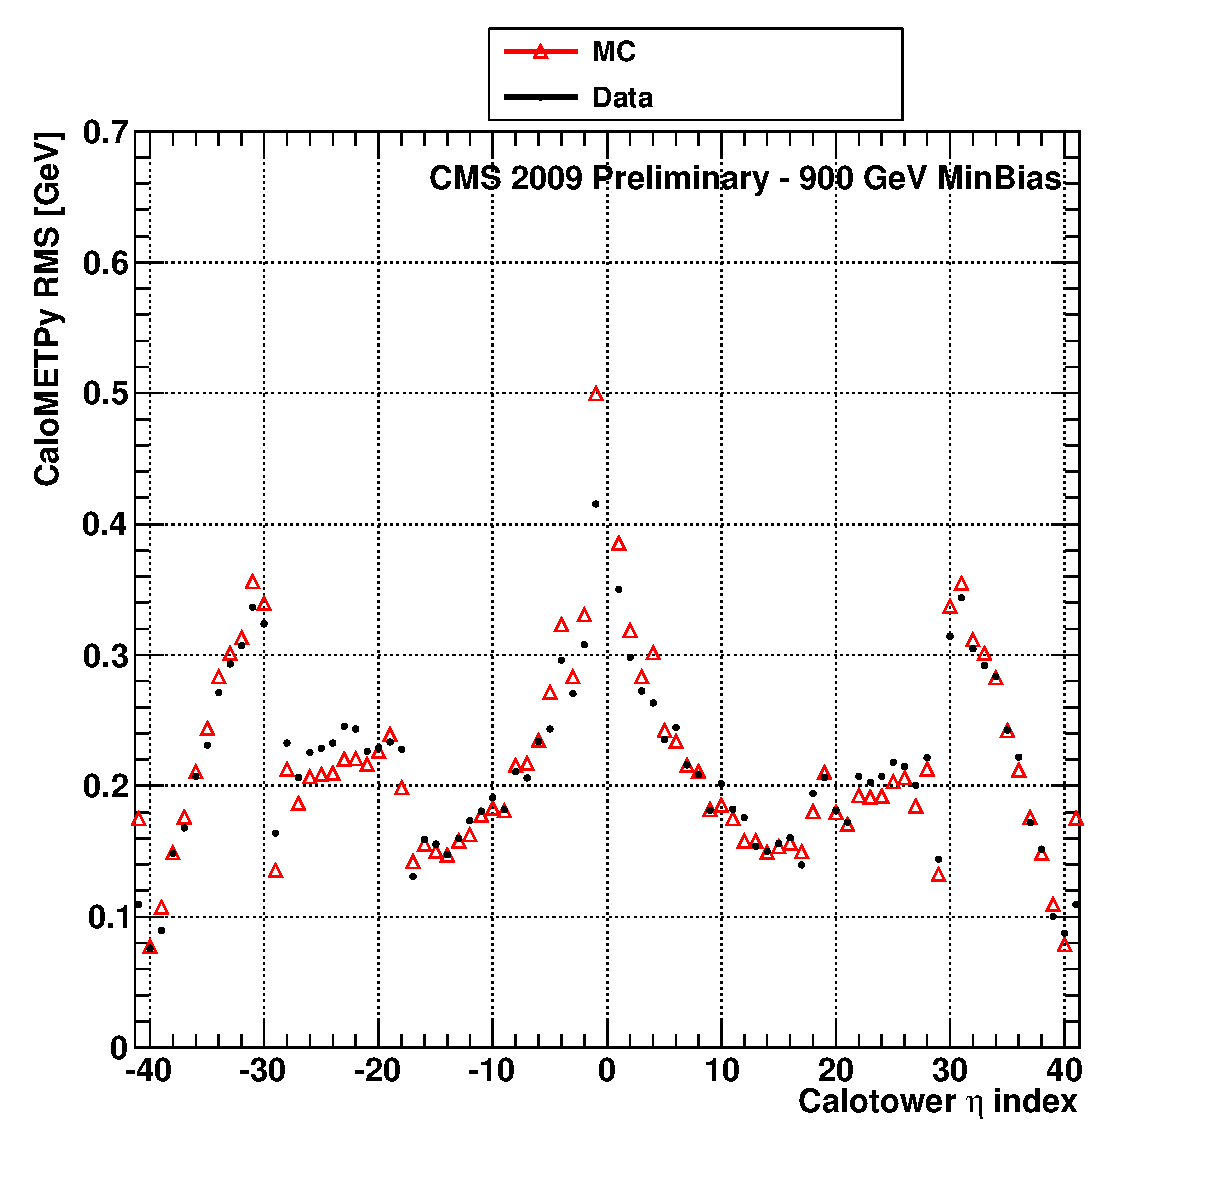
\includegraphics[width=0.5\textwidth]{plots_DataVsMC_MB_900GeV/g_calometPyRMS_vs_ieta_900.eps} \\
 \end{tabular}
 \caption{\small Comparison of the $\eymiss$ Mean vs. i$\eta$ of calotowers and $\eymiss$ RMS vs. i$\eta$ of calotowers between 
          data and Monte Carlo at $900$ GeV.\label{fig:METy_MeanRMS_vs_ieta_900}}
\end{figure}

\clearpage
